\chapter{Neexpandující impulsní gravitační vlny}
V této kapitole se budeme věnovat neexpandujícím impulsním gravitačním vlnám propagujícím se na pozadí Minkowského a (anti-)de Sitterova
prostoročasu. Popíšeme matematickou konstrukci prostoročasů která vede k tzv. refrakčním rovnícím pro geodetiky, které využijeme k vizualizaci různých
řešení impulsních vln a k interpretaci působení vln na různé testovací částice.


\section{Konstrukce}
Nejprve popíšeme konstrukci prostoročasů s neexpandujícíme impulsními gravitačními vlnami
pomocí Penroseovy geometrické metody \cite{Penrose:1972xrn} "cut and paste", zavedeme souřadnice ve
kterých je metrika spojitá a dále se budeme věnovat distribučnímu popisu prostoročasů s impulsními gravitačními
vlnami.

\subsection{"Cut and paste"\ metoda konstrukce}
\label{sec:cut_and_paste_konstrukce1}
Geometrická metoda konstrukce "cut and paste"\ impulsních gravitačních vln v Minkowského prostoročase \eqref{eq:minkowski} se zakládá na rozdělení celého prostoročasu podél rovinné
světelné nadplochy $\mathcal{N}$, kde je implulzní vlna lokalizována na dvě části $\mathcal{M}^+$ a $\mathcal{M}^-$. Opětovným spojením těchto částí a ztotožněním bodů na hranici
řezu $\mathcal{N}$ se specifickým posunutím dostaneme prostoročas s impulsní gravitační vlnou.

\begin{figure}[h]\centering
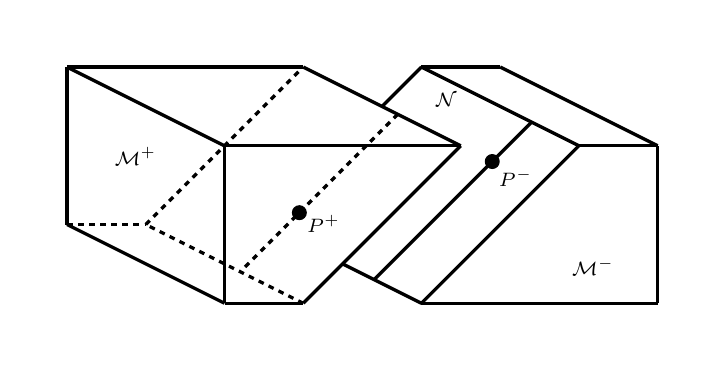
\begin{tikzpicture}
\clip(-2.5,-0.5) rectangle (6.,3.5);
\draw [line width=1.2pt] (-2.,1.)-- (0.,0.);
\draw [line width=1.2pt] (-2.,3.)-- (-2.,1.);
\draw [line width=1.2pt] (0.,0.)-- (0.,2.);
\draw [line width=1.2pt] (0.,2.)-- (-2.,3.);
\draw [line width=1.2pt] (-2.,3.)-- (1.,3.);
\draw [line width=1.2pt] (0.,2.)-- (3.,2.);
\draw [line width=1.2pt] (1.,3.)-- (3.,2.);
\draw [line width=1.2pt] (0.,0.)-- (1.,0.);
\draw [line width=1.2pt] (1.,0.)-- (3.,2.);
\draw [line width=1.2pt,dash pattern=on 2pt off 2pt] (1.,0.)-- (-1.,1.);
\draw [line width=1.2pt,dash pattern=on 2pt off 2pt] (-2.,1.)-- (-1.,1.);
\draw [line width=1.2pt,dash pattern=on 2pt off 2pt] (-1.,1.)-- (1.,3.);
\draw [line width=1.2pt] (2.5,0.)-- (4.5,2.);
\draw [line width=1.2pt] (2.5,0.)-- (5.5,0.);
\draw [line width=1.2pt] (5.5,0.)-- (5.5,2.);
\draw [line width=1.2pt] (4.5,2.)-- (5.5,2.);
\draw [line width=1.2pt] (4.5,2.)-- (2.5,3.);
\draw [line width=1.2pt] (5.5,2.)-- (3.5,3.);
\draw [line width=1.2pt] (2.5,3.)-- (3.5,3.);
\draw [line width=1.2pt] (2.,2.5)-- (2.5,3.);
\draw [line width=1.2pt] (2.5,0.)-- (1.5,0.5);
\draw [line width=1.2pt] (1.9,0.3)-- (3.9,2.3);
\draw [line width=1.2pt,dash pattern=on 2pt off 2pt] (2.2,2.4)-- (0.2,0.4);
\begin{scriptsize}
\draw[color=black] (-1.1302677200189184,1.864045432930641) node {$\mathcal{M}^+$};
\draw[color=black] (2.8186222701156605,2.585603404549911) node {$\mathcal{N}$};
\draw[color=black] (4.6815537604781525,0.46028719723496975) node {$\mathcal{M}^-$};
\draw [fill=black] (0.9503176308657735,1.1503176308657732) circle (2.5pt);
\draw[color=black] (1.2574332042485015,1.0112951028351398) node {$P^+$};
\draw [fill=black] (3.4,1.8) circle (2.5pt);
\draw[color=black] (3.6976110719064135,1.5885414801305562) node {$P^-$};
\end{scriptsize}
\end{tikzpicture}
\caption{Geometrická konstrukce neexpandující impulsní gravitační vlny pomocí metody "cut and paste", 
podél nadplochy $\mathcal{N}$ dojde k rozdělení prostoročasu na dvě části $\mathcal{M}^+$ a $\mathcal{M}^-$ 
a opětovnému ztotožnění bodů na hranici obou částí se specifickým posunem.}
\label{obr01:geomkonstrukt}
\end{figure}

Pro světelnou nadplochu $\mathcal{N}$ danou podmínkou $\mathcal{U}=0$ pak tato konstrukce odpovídá Penroseově 
spojovacím podmínkám

\begin{equation}
    \label{eq:lepici_podminky}
\left[\eta, \bar{\eta}, \mathcal{V}, \mathcal{U}=0_- \right]_{\mathcal{M}^-} \equiv 
\left[\eta, \bar{\eta}, \mathcal{V}-H\left(\eta, \bar{\eta}\right), \mathcal{U}=0_+  \right]_{\mathcal{M}^+},
\end{equation}
kde $H(\eta, \bar{\eta})$ je holomorfní. Penrose \cite{Penrose:1972xrn} ukázal, že impulsní gravitační vlny
jsou v tenzoru křivosti reprezentovány členy proporciálními Diracově delta distribuci $\delta(\mathcal{U})$.
V Minkowského pozadí je nadplocha $\mathcal{U}=0$ rovina a řešení spadá do rodiny impulsních $pp-$vln, tedy
rovnoběžně se propagujících rovinných vln. Obecně na pozadích konstantní křivosti platí stejné napojovací podmínky
\eqref{eq:lepici_podminky} a nadplocha $\mathcal{U}=0$ představuje plochu konstantní Gaussovské křivosti 
$K=\frac{1}{3}\Lambda$ která je popsána metrikou $d\sigma^2=2(1+\frac{1}{6}\Lambda \eta \bar{\eta})^{-2} 
d\eta~d\bar{\eta}$. V případě $\Lambda \neq 0$ se tedy jedná buďto o sféru
($\Lambda > 0$) nebo o hyperbolickou plochu ($\Lambda < 0$). Popis těchto nadploch konstatní křivostsi v (A)dS prostoročasech a
jejich geometrické vlastnosti jsou shrnuty v \cite{Podolsky:1997ri}, kde je také ukázáno,
že se jedná o neexpandující nadplochy.

\begin{figure}[H]
    \centering
    \begin{tikzpicture}
         \node[inner sep=0pt, anchor=south west] (ds) at (0,0)
        {\adjincludegraphics[trim={{.2\width} {.2\height} {.25\width} {.3\height}}, width=.7\textwidth, clip]{../img/kap02/CutAndPaste_NOSUP.pdf}};
    \end{tikzpicture}
    \caption{Nulové geodetiky procházející impulsem nacházejícím se v $\matu=0$ (černá čára) v AdS prostoročase jsou podle cut and paste konstrukce posunuty
    v souřadnici $\matv$ a dochází k refrakci. Geodetiky jsou opět nulovými generátory AdS na $\matu > 0$, neleží už ale v $\eta = 0$ a proto
    neleží na ploše vykresleného hyperboloidu. Světlejší šedá čára odpovídá $\matu = \pm \infty$}
\end{figure}

\subsection{Spojitý tvar metriky}
Metoda "cut and paste"\ nám dává identifikaci bodů prostoročasu na obou stranách impulsní vlny a tedy napojovací podmínky
pro geodetiky, nic ale neříká o podobě metriky kompletního prostoročasu s impulsní vlnou. Potřebujeme tedy najít vhodný
souřadnicový systém, ve kterém bude metrika spojitá funkce $\mathcal{U}$. Toho dosáhneme postupem použitým např. v
\cite{Podolsky:2014ysa}, kde z metriky prostoročasu pozadí \eqref{eq:konfmetric}, respektive
\begin{equation}
    \label{eq:null_background_metric}
    \mathrm{d}s_0^2 = \frac{2~\mathrm{d}\eta~\mathrm{d}\bar{\eta}-2~\mathrm{d}\mathcal{U}~\mathrm{d}\mathcal{V}}
    {\left[1+\frac{1}{6}\Lambda \left(\eta \bar{\eta}
    -\mathcal{U}\mathcal{V}\right)\right]^2},
\end{equation}
souřadnicovou transformací
\begin{equation}
    \label{eq:nonexp_cont_transform}
    \mathcal{U}=U,~~~~ \mathcal{V}=V+H+UH_{,Z}H_{,\bar{Z}},~~~~ \eta=Z+UH_{,\bar{Z}},
\end{equation}
kde uvažujeme libovolnou reálnou funkci $H(Z, \bar{Z})$, obdržíme metriku
\begin{equation}
    \label{eq:nonexp_cont_nokink_metric}
    \mathrm{d} s^{2}=\frac{2\left|\mathrm{d} Z+U\left(H_{, Z \bar{Z}} 
    \mathrm{d} Z+H_{, \bar{Z} \bar{Z}} \mathrm{d} \bar{Z}\right)\right|^{2}-2 \mathrm{d} U 
    \mathrm{d} V}{\left[1+\frac{1}{6} \Lambda(Z \bar{Z}-U V-U G)\right]^{2}}
\end{equation}
kde $G(Z, \bar{Z}) \equiv H - Z H_{,Z}-\bar{Z}H_{,\bar{Z}}$. Metriku \eqref{eq:nonexp_cont_nokink_metric} pak 
uvažujeme pouze pro $U>0$, zatímco na $U<0$ provedeme ztotožnení souřadnic
\begin{equation}
    \label{eq:transformation_just_rename}
    \begin{split}
        &\mathcal{U} = U \\
        &\mathcal{V} = V \\
        &\eta = Z
    \end{split}
\end{equation}
a uvažujeme metriku vzniklou právě touto transformací.
Definováním
tzv. kink funkce jako
\begin{equation}
    \label{eq:kink_function}
    U_+ \equiv U_+(U) = \begin{cases}
        0 & \text{pro } U \leq 0 \\
        U & \text{pro } U \geq 0
    \end{cases}
\end{equation}
můžeme výslednou metriku zapsat jako
\begin{equation}
    \label{eq:nonexp_continuous_metric}
    \mathrm{d} s^{2}=\frac{2\left|\mathrm{d} Z+U_+\left(H_{, Z \bar{Z}} 
    \mathrm{d} Z+H_{, \bar{Z} \bar{Z}} \mathrm{d} \bar{Z}\right)\right|^{2}-2 \mathrm{d} U 
    \mathrm{d} V}{\left[1+\frac{1}{6} \Lambda(Z \bar{Z}-U V-U_+ G)\right]^{2}}.
\end{equation}
Transformace \eqref{eq:nonexp_cont_transform} a \eqref{eq:transformation_just_rename} spojující separátně pro $\mathcal{U}>0$ a $\mathcal{U}<0$ metriku \eqref{eq:null_background_metric}
s metrikou \eqref{eq:nonexp_continuous_metric} lze pomocí Heavisideovy funkce $\Theta(U)$ přepsat do tvaru 
\begin{equation}
    \label{eq:nonexp_cont_full_transform}
    \mathcal{U}=U,~~~~ \mathcal{V}=V+\Theta(U) H + U_+ H_{,Z}H_{,\bar{Z}},~~~~ \eta=Z+ U_+ H_{,\bar{Z}}.
\end{equation}
Stále je ale nutné provádět transformaci separátně pro $\mathcal{U}>0$ a $\mathcal{U}<0$, Heavisideova funkce
má při transformaci metriky \eqref{eq:null_background_metric} za následek vznik členů proporcionálních delta funkci.
Ukazuje se, že tato transformace spojuje tzv. distribuční vyjádření metriky \eqref{eq:nonexp_distr_metric_omega}, které bude zavedeno dále,
se spojitým tvarem metriky \eqref{eq:nonexp_continuous_metric}.
Transformace \eqref{eq:nonexp_cont_full_transform} zároveň obsahuje Penroseovy spojovací podmínky \eqref{eq:lepici_podminky} v $U=0$, kde
vzniká nespojitost v souřadnici $\mathcal{V}$. Tato metoda konstrukce tedy představuje explicitní "cut and paste"\ konstrukci.


\subsection{Distribuční tvar metriky}
Dalším způsobem konstrukce impulsní gravitační vlny je přechod od příslušných rodin tzv. "sandwichových"\
gravtiačních vln s hladkým profilem vlnoplochy k limitnímu distribučnímu vyjádření impulsní vlny. Pro případ neexpandujícíh vln, propagujících se
na $\mathbb{E}^{1,3}$, byl tento limitní přechod uvažován např. v \textcolor{red}{citace, citace, citace...}, výsledná metrika
nabývá tvaru
\begin{equation}
    \rmd s^2 = 2~ \rmd \xi \rmd \bar{\xi} - 2 \rmd u \rmd v + H(\xi, \bar{\xi}) \delta\left( u\right) \rmd u^2
\end{equation}


Distribuční tvar metriky také dostaneme dosazením invezní transformace k \eqref{eq:nonexp_cont_full_transform} do spojité metriky 
\eqref{eq:nonexp_continuous_metric}. Vzhledem k nespojitosti v transformaci toto dosazení nemůže být provedeno
v rámci klasické teorie distribucí, kde nelze konzistentně definovat násobení dvou distribucí. S využitím regularizačních metod teorie
nelineárních zobecněných funkcí \textcolor{red}{zde citace}, které zakládají na Colombeaových algebrách, lze ale odvodit pravidla pro násobení
jisté třídy distribucí, která dostačují pro toto odvození. Konkrétně potřebujeme násobit distribuce
\begin{equation}
        \Theta^2 = \Theta, ~~~~ \Theta U_{+} = U_{+}.
\end{equation}
Kromě pravidel pro násobení ještě využijeme identity z klasické teorie distribucí
\begin{equation}
    \Theta' = \delta, ~~~~ U_{+}' = \Theta
\end{equation}
a dostáváme metriku ve tvaru
\begin{equation} \label{eq:nonexp_distr_metric_omega}
\mathrm{d}s^2=\frac{2\mathrm{d}\eta~\mathrm{d}\bar{\eta} - 2 \mathrm{d}\mathcal{U}~\mathrm{d}\mathcal{V} + 2H(\eta, \bar{\eta}) \delta(\mathcal{U}) 
~\mathrm{d}\mathcal{U}^2}{\left[1+\frac{1}{6}\Lambda(\eta \bar{\eta}-\mathcal{U}\mathcal{V})\right]^2}.
\end{equation}

V případě nenulové kosmologické konstanty můžeme také využít vnoření do $\mathbb{E}^{1,4}$, případně $\mathbb{E}^{2,4}$ (podle znaménka kosmologické
konstanty, jak je popsáno v kapitole\autoref{chap:kap01}) s dodatečným neexpandujícím impulsem
\begin{equation}
    \label{eq:5DDistributionalWaveMetric}
    \rmd s^2 = \rmd Z_2^2 \rmd Z_3^2 + \epsilon \rmd Z_4^2 - 2 \rmd \tilde{U} \rmd \tilde{V} + \mathcal{H}(Z_2, Z_3, Z_4) \delta(\tilde{U}) \rmd \tilde{U}^2,
\end{equation}
kde $\epsilon = \text{sign} (\Lambda)$, $\tilde{U} = \tfrac{1}{\sqrt{2}}(Z_0 + Z_1)$, $\tilde{V}= \tfrac{1}{\sqrt{2}}(Z_0-Z_1)$.
S podmínkou analogickou k \eqref{eq:dS_hyperboloid} a \eqref{eq:AdS_hyperboloid},
\begin{equation}
    Z_2^2 + Z_3^2 + \epsilon Z_4^2 - 2 \tilde{U} \tilde{V} = \epsilon a^2,
\end{equation}
dostáváme reprezentaci impulsních vln propagujících se na (A)dS prostoročasu s impulsem na $\tilde{U}=0$ \cite{Podolsky1997}.
Funkce $H$ a $\mathcal{H}$ v metrikách \eqref{eq:nonexp_distr_metric_omega} a \eqref{eq:5DDistributionalWaveMetric} jsou svázány vztahem
\begin{equation}
    \mathcal{H} = \frac{2H}{1+\frac{1}{6}\Lambda \eta \bar{\eta}}
\end{equation}


\section{Interakce s testovacími částicemi}

\subsection{Profil impulsní gravitační vlny}
\textcolor{red}{Toto bych raději přejmenoval jinak}
Pro distribuční metriku \eqref{eq:nonexp_distr_metric_omega} se Einsteinovy rovnice \eqref{eq:einsten_field_equations} pro nulovou pravou stranu redukují na
\begin{equation}
    \label{eq:podminka_na_H_lambda}
    \left(\Delta + \frac{2}{3} \Lambda \right)\mathcal{H} = 0,
\end{equation}
pro případ nulové kosmologické konstanty dostáváme
\begin{equation}
    \label{eq:podminka_na_H}
    \Delta H = 2 H_{,\eta \bar{\eta}} = 0.
\end{equation}

Konkrétní tvar $H=2\mu \log(\eta \bar{\eta})$ pro prostoročas s $\Lambda=0$ odvodili Aichelburg a Sexl \cite{Aichelburg_1971} pomocí limitního boostu ($v \to c$)
Schwrazschildova řešení při $m \to 0$, aby byla hodnota $\mu = m(1-v^2)^{-1/2}$ konstantní.
Zobecnění na (anti-)de Sitterův prostoročas provedli Hotta a Tanaka \cite{Hotta_1993} 
boostem Schwarzschildova- (anti-) de Sitterova prostoročasu. Aichelburg-Sexlovo řešení představuje gravitační vlnu generovanou
nulovou částicí v $\eta = 0$, Hottovo-Tanakovo řešení pak v de Sitterově prostoročasu odpovídá dvěma, opačným směrem letícím, nulovým částicím,
které generují neexpandující sférickou gravitační vlnu, v anti-de Sitterově prostoročasu (ve kterém existují uzavřené časupodobné křivky) impulsní vlnu generovanou nulovou částicí
která v nekonečném cyklu prolétává z jedné strany vesmíru na druhou.

Griffiths a Podolský v článcích \cite{Griffiths_1997} a \cite{Podolsky1997} využili \eqref{eq:podminka_na_H}, resp. \eqref{eq:podminka_na_H_lambda}
ke zkonstruování obecnějšího tvaru funkce $H$, resp. $\mathcal{H}$, kde je neexpandující gravitační vlna generována
nulovými částicemi s libovolnou multipólovou strukturou.

\subsection{Refrakční rovnice}
V článku \cite{Podolsky:2014ysa} Podolský, Säamann, Steinbauer a Švarc \textcolor{red}{dopsat o C1 matchingu (Filippov, existence úplných C1 geodetik v spojitých souřadnicích)}


Změna polohy (nalepení geodetiky) je dána Penroseovými spojovacími podmínkami, tento skok ale generuje změnu v derivacích poloh a dojde tedy
k refrakci geodetik na impulsní nadploše $\mathcal{U}=0$ podle tzv. refrakčních rovnic
\begin{align}
    \label{eq:refraction_nonexpanding}
    \begin{split}
        &\dot{\mathcal{U}}^{+}_{\mathrm{i}} = \dot{\mathcal{U}}^{-}_{\mathrm{i}}\\
        &\dot{\mathcal{V}}^{+}_{\mathrm{i}} = \dot{\mathcal{V}}_{\mathrm{i}}^{-} + H_{\mathrm{i}, Z}
        \dot{\eta}^{-}_{\mathrm{i}} + H_{\mathrm{i}, \bar{Z}} \dot{\overline{\eta}}^{-}_{\mathrm{i}} + 
        H_{\mathrm{i}, Z} H_{\mathrm{i}, \bar{Z}} \dot{\mathcal{U}}_{\mathrm{i}}^{-}\\
        &\dot{\eta}_{\mathrm{i}}^{+} =\dot{\eta}_{\mathrm{i}}^{-}+H_{\mathrm{i}, \bar{Z}}
        \dot{\mathcal{U}}_{\mathrm{i}}^{-}.
    \end{split}
\end{align}
Index $i$ znamená hodnotu na impulsní nadploše, složky označené znakem + jsou za impulsem a tedy v části prostoročasu $\mathcal{M}^+$,
složky označené znakem - jsou před impulsem v $\mathcal{M}^-$.


\subsection{Vizualizace}
\textcolor{red}{Zde vykreslené obrázky s popisem, jak pro světelné částice tak pro
časupodobné geodetiky (případně i pro srandu prosoturupodobné)}
